\mode*

\begin{frame}
  \tableofcontents
\end{frame}

\section{Disposition}

\begin{frame}
  \begin{enumerate}
    \item What makes humans human?
      \hfill
      (forms of learning)
    \item What is to be learned?
      \hfill
      (learning objectives)
    \item Sameness and difference in learning
      \hfill
      (variation theory)
    \item What does the world look like to others?
      \hfill
      (phenomenography)
    \item The art of learning
      \hfill
      (learning alone, doing research)
    \item Making learning possible
      \hfill
      (teaching)
    \item Learning to help others to learn
      \hfill
      (education research)
  \end{enumerate}
\end{frame}


\section{Theory}

\begin{frame}
  \begin{enumerate}
    \item What makes humans human?
      \hfill
      (forms of learning)
    \alert{
    \item What is to be learned?
      \hfill
      (learning objectives)
    }
    \item Sameness and difference in learning
      \hfill
      (variation theory)
    \item What does the world look like to others?
      \hfill
      (phenomenography)
    \item The art of learning
      \hfill
      (learning alone, doing research)
    \item Making learning possible
      \hfill
      (teaching)
    \item Learning to help others to learn
      \hfill
      (education research)
  \end{enumerate}
\end{frame}

\begin{frame}
  \begin{block}{Ch 2 What is to be learned?}
    \begin{itemize}
      \item What is an intended learning outcome?
      \item What should it be?
      \item It depends on the learner: \emph{critical aspects, critical 
        features} --- the atoms of the learning objective.
    \end{itemize}
  \end{block}

  \pause

  \begin{block}{The goal}
    \begin{itemize}
      \item \textcquote{NecessaryConditionsOfLearning}{The focus of the theory 
        elaborated in this book is on learning to handle new situations in 
      powerful ways.}
    \end{itemize}
  \end{block}
\end{frame}

\begin{frame}
  \begin{figure}
    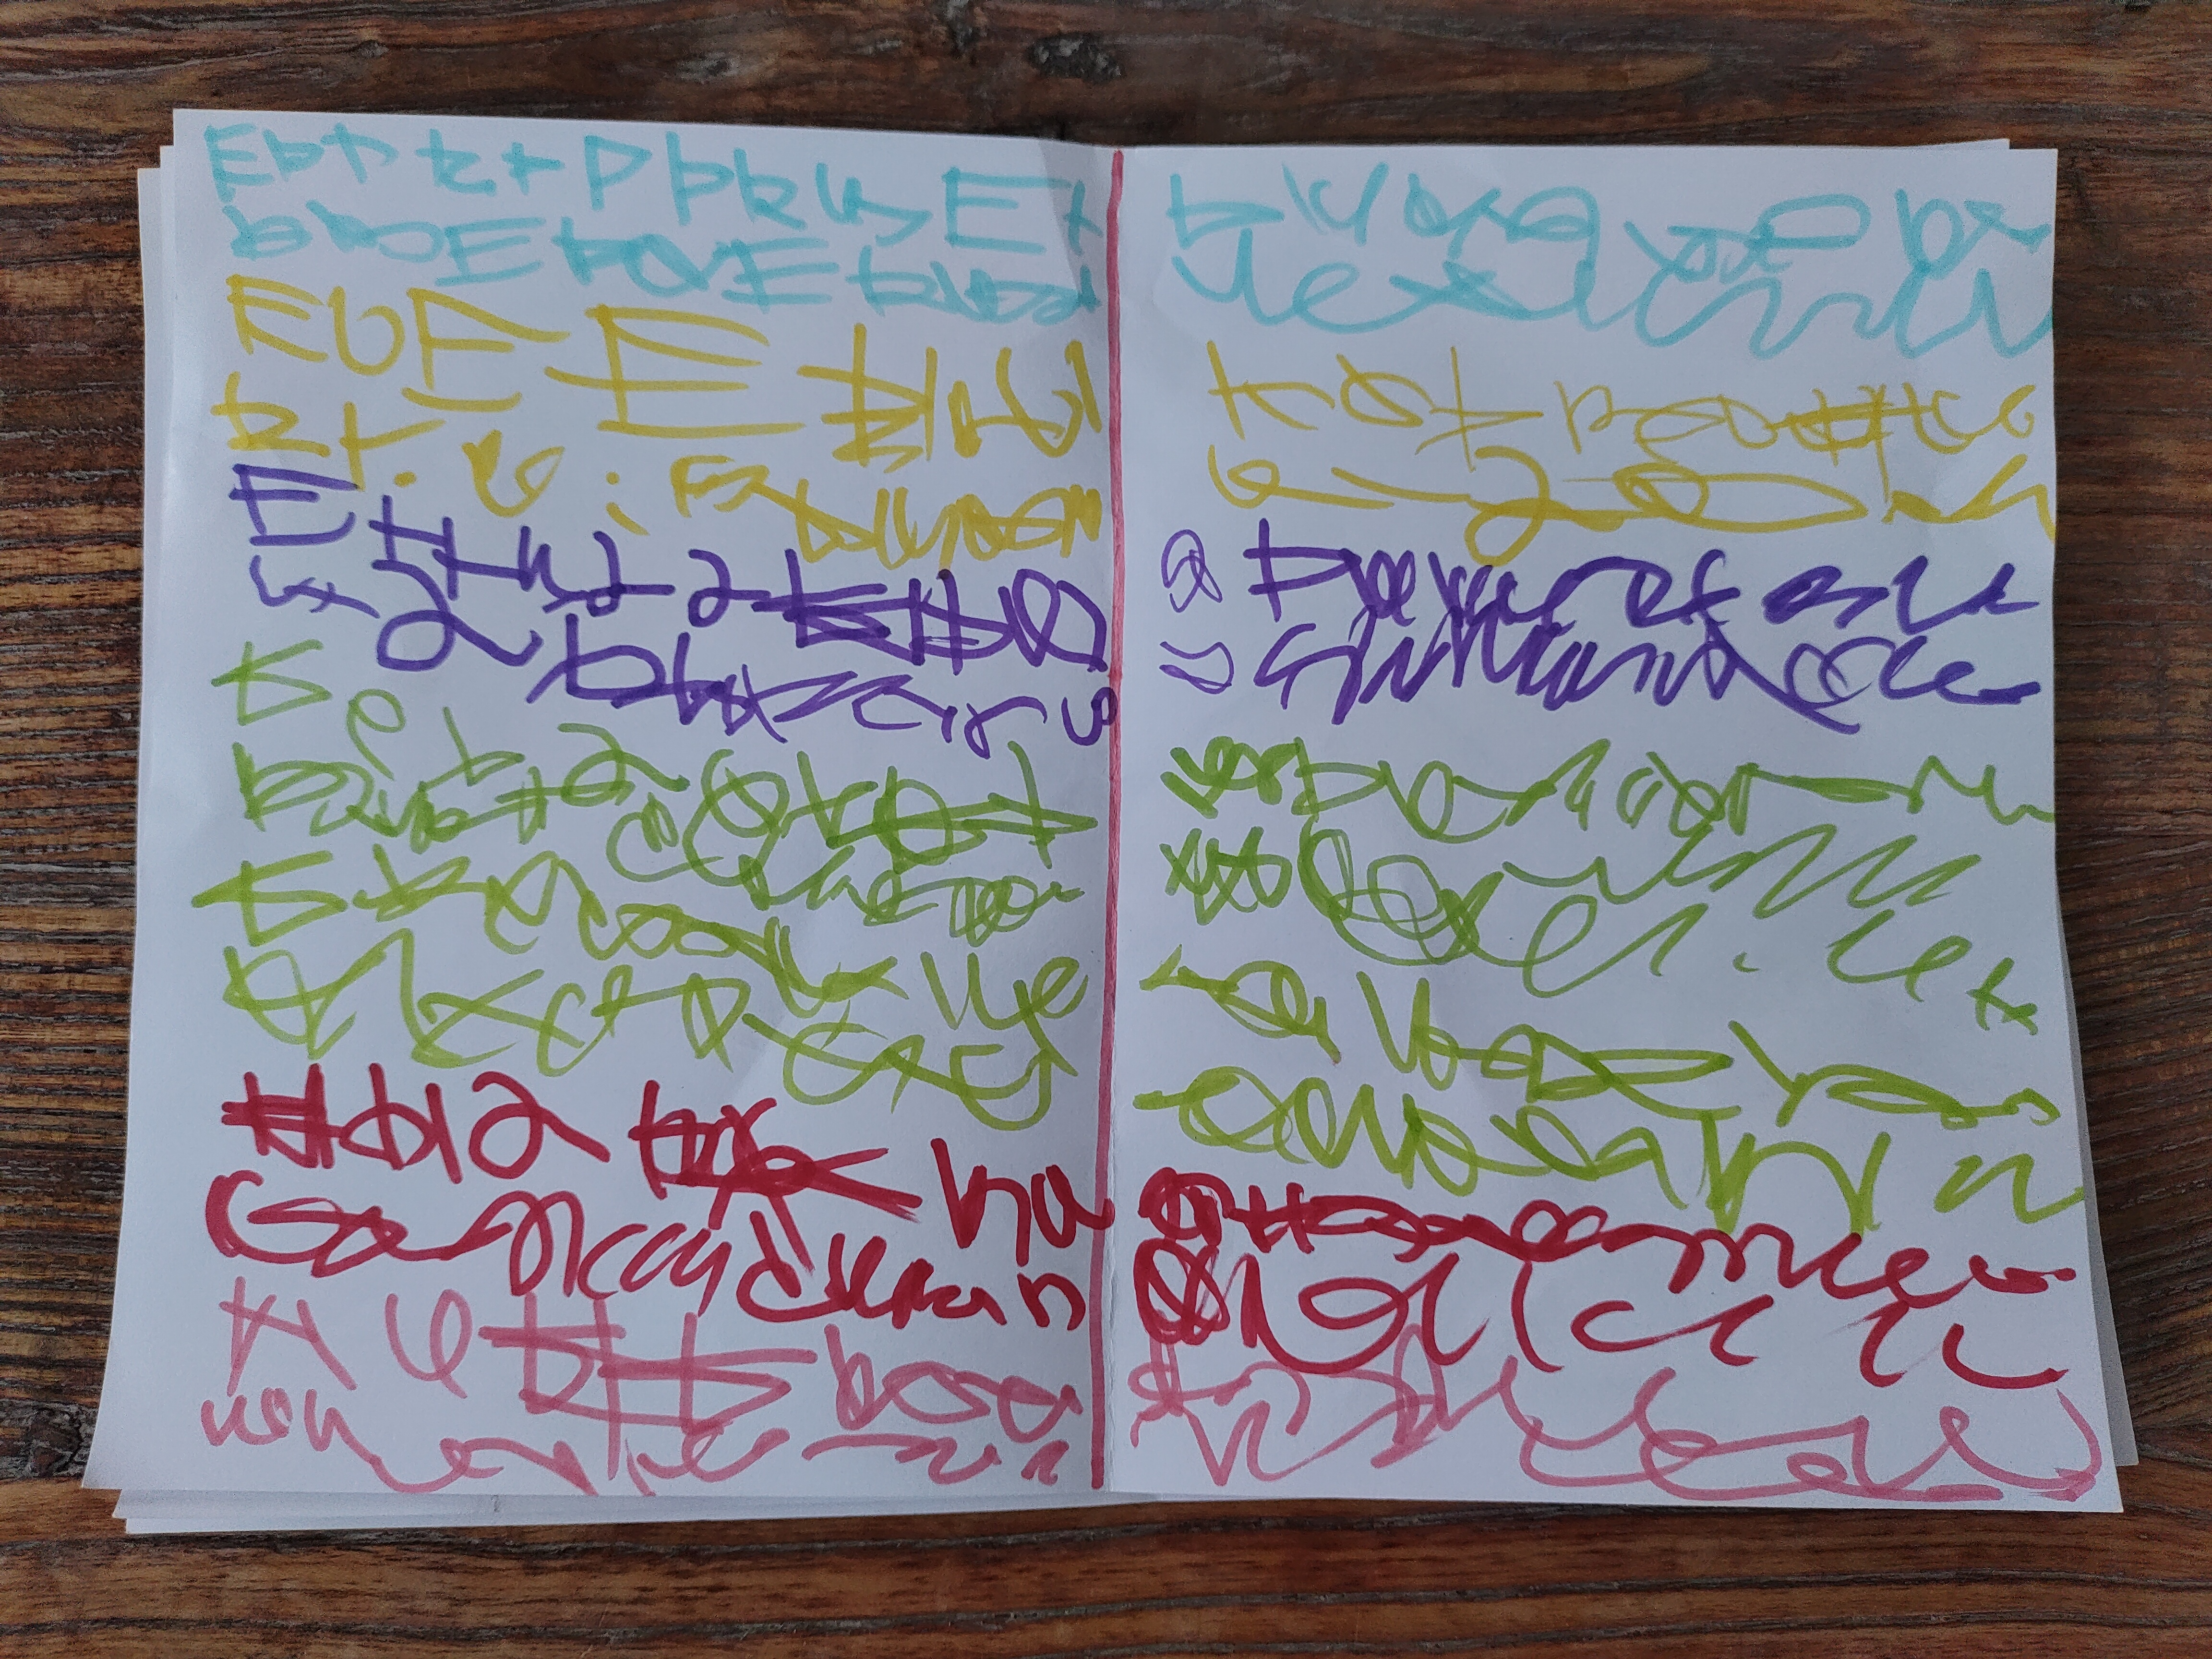
\includegraphics[height=0.5\textheight]{fig/maja-writing.jpg}
    \caption{Child's writing.
      (Corresponds to~\cite[Fig.~2.1, p.~30]{NecessaryConditionsOfLearning}.)
    }
  \end{figure}
  \begin{example}
    \begin{itemize}
      \item Obviously knows some aspect(s) of writing, just not all.
      \item Even the camera app detected this as text.
    \end{itemize}
  \end{example}
\end{frame}

\begin{frame}[fragile]\label{vtprogid}
  \begin{example}[Functions in Python]
    \lstexample{examples/greet.py}
  \end{example}

  \begin{example}[Aspects of functions]
    \begin{columns}
      \begin{column}{0.4\columnwidth}
        \begin{itemize}
          \item Variable scope
          \item Argument order
        \end{itemize}
      \end{column}
      \begin{column}{0.5\columnwidth}
        \begin{itemize}
          \item Call stack (\enquote{execution flow})
          \item Return values
        \end{itemize}
      \end{column}
    \end{columns}
  \end{example}
\end{frame}


\begin{frame}
  \begin{enumerate}
    \item What makes humans human?
      \hfill
      (forms of learning)
    \item What is to be learned?
      \hfill
      (learning objectives)
    \alert{
    \item Sameness and difference in learning
      \hfill
      (variation theory)
    }
    \item What does the world look like to others?
      \hfill
      (phenomenography)
    \item The art of learning
      \hfill
      (learning alone, doing research)
    \item Making learning possible
      \hfill
      (teaching)
    \item Learning to help others to learn
      \hfill
      (education research)
  \end{enumerate}
\end{frame}

\begin{frame}
  \begin{block}{Ch 3 Sameness and difference in learning}
    \begin{itemize}
      \item The problem with direct reference (induction).
      \item The patterns: contrast, generalization, fusion.
      \item \textcquote[p.~71]{NecessaryConditionsOfLearning}{%
          \textins{P}racticing something other than what was tested was more 
          effective than practicing exactly what was tested.%
        }
    \end{itemize}
  \end{block}

  \begin{example}<2>[Using known to prepare for unknown, 
    {\cite[pp.~67--71]{NecessaryConditionsOfLearning}}]
    \begin{itemize}
      \item Kids were to hit a target by throwing a shuttlecock (badminton 
        \enquote{ball}).
    \end{itemize}
    \begin{enumerate}
      \item Practicing from the same position as testing.
      \item Practicing from several positions, \emph{except the testing 
        position}.
    \end{enumerate}
  \end{example}
\end{frame}

\begin{frame}
  \begin{figure}
    \begin{subfigure}{0.3\columnwidth}
      \centering
      \includegraphics{fig/contrast-color.tikz}
      \caption{Contrast}
    \end{subfigure}
    \hfill
    \begin{subfigure}{0.3\columnwidth}
      \centering
      \includegraphics{fig/generalization-color.tikz}
      \caption{Generalization}
    \end{subfigure}
    \hfill
    \begin{subfigure}{0.3\columnwidth}
      \centering
      \includegraphics{fig/fusion-color.tikz}
      \caption{Fusion}
    \end{subfigure}
    \caption{%
      Illustrating the patterns of variation for aspects color and shape.
    }
  \end{figure}

  \begin{onlyenv}<1>
    \begin{example}
      \begin{itemize}
        \item Critical aspect: colour.
        \item Critical feature: blue.
        \item Non-critical feature: green.
        \item Non-critical aspect: shape.
        \item Non-critical features: circle, square.
      \end{itemize}
    \end{example}
  \end{onlyenv}
  \begin{onlyenv}<2>
    \begin{remark}
      \begin{itemize}
        \item There are other aspects too, \emph{unintentionally}.
        \item Another aspect in this figure is order: the circle is always 
          \enquote{first} (to the right).
      \end{itemize}
    \end{remark}
  \end{onlyenv}
\end{frame}

\begin{frame}
  \begin{example}[Physics, {\cite[p.~58]{NecessaryConditionsOfLearning}}]
    \begin{enumerate}
      \item Students were introduced to modern physics.
      \item Students were introduced to modern physics, contrasted with what we 
        believed before.
    \end{enumerate}
  \end{example}
\end{frame}

\begin{frame}[fragile]\label{vtprogid}
  \begin{example}[One aspect of functions: scope]
    \lstexample{examples/greet.py}
  \end{example}

  \begin{block}{Output}
    \runexample{examples/greet.py}
  \end{block}
\end{frame}

\begin{frame}[fragile]\label{vtprogidcon}
  \begin{example}[Contrast identifiers in different scopes]
    \lstexample[highlightlines=5-7]{examples/scope-contrast.py}
  \end{example}

  \begin{block}{Output}
    \runexample{examples/scope-contrast.py}
  \end{block}
\end{frame}

\begin{frame}[fragile]
  \begin{example}[Contrast identifiers in different scopes]
    \lstexample[highlightlines=5]{examples/scope-contrast-more.py}
  \end{example}

  \begin{block}{Output}
    \runexample{examples/scope-contrast-more.py}
  \end{block}
\end{frame}

\begin{frame}[fragile]\label{vtprogord}
  \begin{example}[Another aspect: argument order]
    \lstexample{examples/greet.py}
  \end{example}

  \begin{block}{Output}
    \runexample{examples/greet.py}
  \end{block}
\end{frame}

\begin{frame}[fragile]\label{vtprogordcon}
  \begin{example}[Constrast argument order]
    \lstexample[highlightlines={1,7}]{examples/order-contrast.py}
  \end{example}

  \begin{block}{Output}
    \runexample{examples/order-contrast.py}
  \end{block}
\end{frame}

%\begin{frame}[fragile]\label{vtprogordcon}
%  \begin{example}[Function default arguments]
%    \lstexample{examples/default.py}
%  \end{example}
%
%  \begin{block}{Output}
%    \runexample{examples/default.py}
%  \end{block}
%\end{frame}

\begin{frame}
  \begin{enumerate}
    \item What makes humans human?
      \hfill
      (forms of learning)
    \item What is to be learned?
      \hfill
      (learning objectives)
    \item Sameness and difference in learning
      \hfill
      (variation theory)
    \alert{
    \item What does the world look like to others?
      \hfill
      (phenomenography)
    }
    \item The art of learning
      \hfill
      (learning alone, doing research)
    \item Making learning possible
      \hfill
      (teaching)
    \item Learning to help others to learn
      \hfill
      (education research)
  \end{enumerate}
\end{frame}

\begin{frame}
  \begin{block}{Ch 4 What does the world look like to others?}
    \begin{itemize}
      \item This chapter is about phenomenography.
      \item It answers the question \enquote{how can we find out what things 
        look like to other people?}
      \item Also tells us something about assessment\footnote{%
          Marton contrasts Bloom and SOLO taxonomies and phenomenography.
        } and how to find those critical aspects.
    \end{itemize}
  \end{block}

  \pause

  \begin{example}
    \begin{itemize}
      \item \textcquote[pp.~112--113]{NecessaryConditionsOfLearning}{%
          \textins{U}nderstanding does not cause acts; instead, acts express 
          understanding.%
        }
    \end{itemize}
  \end{example}
\end{frame}

\begin{frame}
  \begin{remark}[Philosophical/theoretical view]
    \begin{itemize}
      \item No one sees the world \enquote{as it is}.
      \item The world is viewed from one's own \emph{perspective}, always 
        through the lens of the self.
      \item \emph{The learner should learn to view things in more powerful 
        ways.}
    \end{itemize}
  \end{remark}

  \pause

  \begin{remark}
    \begin{itemize}
      \item Another \emph{view} of this is \enquote{mental models}.
    \end{itemize}
  \end{remark}
\end{frame}

\begin{frame}
  \begin{remark}[Assessment]
      \textcquote[p.~89]{NecessaryConditionsOfLearning}{%
          If we want to find out to what extent they have learned to do so, we 
          should not point out those aspects for them but let the students 
          discern them by themselves.
          Only then might we be able to find out how they deal with novel 
          situations, how they handle the unknowns by the means of the known.%
        }
  \end{remark}
\end{frame}

\begin{frame}
  \begin{example}[Newton's first law, nationellt prov in physics, year 11]
    \textcquote[p.~90]{NecessaryConditionsOfLearning}{%
      In an experiment with a ball, it is found that when the ball falls, it is 
      affected by the air braking force \(F\), which is proportional to the 
      velocity of the ball, \(v\), that is \(F = kv\) where \(k\) in this case 
      is \SI{0.32}{\newton\second\per\metre}. What would the final velocity of 
      the ball be if it were dropped from a high altitude?
      The ball's mass is \SI{0.20}{\kilogram}.%
    }
  \end{example}

  \pause

  \begin{remark}
    \begin{itemize}
      \item \textcquote[p.~90]{NecessaryConditionsOfLearning}{%
          The learners do not have to discern what aspects of the event have to 
          be taken into consideration: they all are pointed out in the 
          problem.%
        }
      \item They must know the gravitational force, \(mg\).
    \end{itemize}
  \end{remark}
\end{frame}

\begin{frame}
  \begin{example}[Newton's first law; Johansson, Marton, Svensson 1985]
    \textcquote[p.~91]{NecessaryConditionsOfLearning}{%
      A car is driven at a high constant speed on a motorway.
      What forces act on the car?
    }
  \end{example}

  \pause

  \begin{remark}
    \begin{itemize}
      \item Relates back to the \enquote{Teacher's Paradox} (Ch 1).
      \item \textcquote[p.~13]{NecessaryConditionsOfLearning}{%
          \textins{T}he more clearly the teacher tells the students what is 
          to be done, the less chance the students get to make the necessary 
          distinctions (for instance, between what is critical and what is 
          not).%
        }
    \end{itemize}
  \end{remark}
\end{frame}


\section{Theory in practice}

\begin{frame}
  \begin{enumerate}
    \item What makes humans human?
      \hfill
      (forms of learning)
    \item What is to be learned?
      \hfill
      (learning objectives)
    \item Sameness and difference in learning
      \hfill
      (variation theory)
    \item What does the world look like to others?
      \hfill
      (phenomenography)
    \alert{
    \item The art of learning
      \hfill
      (learning alone, doing research)
    }
    \item Making learning possible
      \hfill
      (teaching)
    \item Learning to help others to learn
      \hfill
      (education research)
  \end{enumerate}
\end{frame}

\begin{frame}
  \begin{block}{Ch 5 The art of learning}
    \begin{itemize}
      \item How do people do to learn new things?
      \item Deep and surface learning
      \item Scientific discoveries as learning
    \end{itemize}
  \end{block}

  \pause

  \begin{example}[{\cite[p.~129]{NecessaryConditionsOfLearning}}]
    \begin{itemize}
      \item Children naturally generate the necessary patterns of variation and 
        invariance.
    \end{itemize}
  \end{example}

  \pause

  \begin{question}
    \begin{itemize}
      \item Do we kill that ability in the (Western) school system?
    \end{itemize}
  \end{question}
\end{frame}

\begin{frame}
  \begin{remark}
    \textcquote[p.~147]{NecessaryConditionsOfLearning}{%
      How we learn and what we learn are fundamentally intertwined.%
    }
  \end{remark}

  \begin{example}[Deep and surface learning, 
    {\cite[pp.~142--147]{NecessaryConditionsOfLearning}}]
    \begin{description}
      \item[Surface] try to memorize.
      \item[Deep] generate patterns of variation and invariance for oneself.
    \end{description}
  \end{example}
\end{frame}

\begin{frame}
  \begin{enumerate}
    \item What makes humans human?
      \hfill
      (forms of learning)
    \item What is to be learned?
      \hfill
      (learning objectives)
    \item Sameness and difference in learning
      \hfill
      (variation theory)
    \item What does the world look like to others?
      \hfill
      (phenomenography)
    \item The art of learning
      \hfill
      (learning alone, doing research)
    \alert{
    \item Making learning possible
      \hfill
      (teaching)
    }
    \item Learning to help others to learn
      \hfill
      (education research)
  \end{enumerate}
\end{frame}

\begin{frame}
  \begin{block}{Ch 6 Making learning possible}
    \begin{itemize}
      \item How can we use this theory for teaching?
      \item Covers differences between cultures.
      \item Covers many studies on teaching.
      \item Direct teaching vs learning by discovery
    \end{itemize}
  \end{block}
\end{frame}

\begin{frame}
  \begin{example}[Teaching in US and Japan,
    {\cite[pp.~181--183]{NecessaryConditionsOfLearning}}]
    \begin{description}
      \item<1,3->[US classrom] Teacher introduces method for solving a type of 
        problem.
        After demonstration, students solve problems of this kind.

      \item<2,3->[Japanese classroom] Teacher introduces complex problem.
        Students have a go at it.
        Discuss approaches in full class.
        \alert<5>{\onslide<5>{Then practice.}}
    \end{description}
  \end{example}

  \begin{uncoverenv}<3->
    \begin{table}
      \caption{Comparison of patterns of variation.}
      \begin{tabular}{llll}
        \toprule
        \multicolumn{2}{c}{American} &
        \multicolumn{2}{c}{Japanese} \\
        \midrule
        method & \alert<4>{problem} & \alert<4>{method} & \alert<5>{problem} \\
        invariant & \alert<4>{varies} &
        \alert<4>{\only<1-4>{varies}\only<5>{invariant}} &
        \alert<5>{\only<5>{varies}\only<1-4>{invariant}} \\
        \bottomrule
      \end{tabular}
    \end{table}
  \end{uncoverenv}
\end{frame}

\begin{frame}
  \begin{example}[{\enquote{One thing at a time}},
    {\cite[pp.~166--168]{NecessaryConditionsOfLearning}}]
    \begin{itemize}
      \item Medical students learning about ECGs.
      \item Three types of heart failures.
    \end{itemize}
    \begin{description}
      \item[Group A] Lecture (two cases/category), tutorial (12 cases,
        \alert<2->{groups of 4, one failure type at a time})
      \item[Group B] Lecture (two cases/category), tutorial (12 cases,
        \alert<2->{all at once})
    \end{description}
    \begin{itemize}
      \item<3> Group B did \emph{more than 50\% better} than Group A.
    \end{itemize}
  \end{example}
\end{frame}

\begin{frame}
  \begin{remark}
    \begin{itemize}
      \item One thing at a time: \emph{dimension}
      \item Things together: \emph{features} in the dimension
    \end{itemize}
  \end{remark}

  \pause

  \begin{remark}
    \begin{enumerate}
      \item How cases are organized (ECG outputs, iterations)
      \item Differences as change (dynamic visualization, deriving a formula)
    \end{enumerate}
  \end{remark}
\end{frame}


\section{Summary}

\begin{frame}
  \begin{example}[The patterns]
    \begin{enumerate}
      \item \alert<1>{Undivided whole}
      \item \alert<2>{Discern parts}: \alert<3>{contrast} + 
        \alert<4>{generalization}
      \item Put parts back together: \alert<5>{fusion}
    \end{enumerate}
  \end{example}

  \begin{figure}
    \includegraphics{fig/part-whole.tikz}
  \end{figure}

  \begin{onlyenv}<6-7>
    \begin{remark}
      \begin{itemize}
        \item<6> Can be applied to a course, lecture, lab or research paper.
        \item<7> This is applied recursively to every part.
      \end{itemize}
    \end{remark}
  \end{onlyenv}

  \begin{onlyenv}<8>
    \begin{remark}[An implication]
      \begin{itemize}
        \item The \emph{general} is part of the \emph{special case}.
        \item Not the other way around.
      \end{itemize}
    \end{remark}
  \end{onlyenv}
\end{frame}


\section{Exercise time}

\begin{frame}
  \begin{exercise}[Analyse teaching material]
    \begin{enumerate}
      \item What is the educational objective?
        \begin{itemize}
          \item What are the critical aspects?
          \item What are the students assumed to already know?
        \end{itemize}
      \item What patterns of variations did you use and how?
        \begin{itemize}
          \item What aspects are you thus focusing and when?
          \item Will the students be able to learn?
        \end{itemize}
      \item How should you adapt the patterns of variation to improve?
    \end{enumerate}
  \end{exercise}
\end{frame}

\section{Research}

\begin{frame}
  \begin{enumerate}
    \item What makes humans human?
      \hfill
      (forms of learning)
    \item What is to be learned?
      \hfill
      (learning objectives)
    \item Sameness and difference in learning
      \hfill
      (variation theory)
    \item What does the world look like to others?
      \hfill
      (phenomenography)
    \item The art of learning
      \hfill
      (learning alone, doing research)
    \item Making learning possible
      \hfill
      (teaching)
    \alert{
    \item Learning to help others to learn
      \hfill
      (education research)
    }
  \end{enumerate}
\end{frame}

\begin{frame}
  \begin{block}{Ch 7 Learning to help others to learn}
    \begin{itemize}
      \item How can teachers learn to be better teachers?
      \item Learn to handle the objects of learning in powerful ways.
      \item Must find out what the learner needs to learn to see.
    \end{itemize}
  \end{block}

  \pause

  \begin{remark}[Chapter 2, object of learning]
    \begin{description}
      \item[Educational objective]
        What the learners are expected to become able to to do.

      \item[Critical aspects to discern]
        What they need to learn in order to achieve this.
    \end{description}
  \end{remark}
\end{frame}

\begin{frame}
  \begin{remark}
    \begin{itemize}
      \item<+> \textcquote[p.~255]{NecessaryConditionsOfLearning}{%
          Knowing what the learner is supposed to become able to do does not 
          suggest what we should do in order to help the learner to learn.%
        }
      \item<+> \textcquote[p.~255]{NecessaryConditionsOfLearning}{%
          For this, we must find out what the learner needs to learn to see.%
        }
    \end{itemize}
  \end{remark}
\end{frame}

\begin{frame}
  \begin{example}[What is to be 
    done~{\cite[p.~257]{NecessaryConditionsOfLearning}}, part I]
    \begin{enumerate}
      \item<+> Choose a learning target (specify what the students are expected 
        to be able to do by the end of the unit).
      \item<+> Find out what the learners can do already and what they must 
        learn in order to achieve the target (find the critical aspects).
      \item<+> Identify the pattern of variation and invariance that is 
        necessary for the learners to discern the critical aspects of the 
        object of learning and to focus on them simultaneously.
      \item<+> Find out what the learners have to do in order to appropriate 
        the object of learning; that is, find out in what kind of activities 
        the pattern of variation and invariance should be embedded.
        \saveenumi
    \end{enumerate}
  \end{example}
\end{frame}

\begin{frame}
  \begin{example}[What is to be 
    done~{\cite[p.~257]{NecessaryConditionsOfLearning}}, part II]
    \begin{enumerate}
      \resumeenumi
      \item<+> Carry out the plan, adjusting it continuously.
      \item<+> Find out what the students have learned.
      \item<+> Draw conclusions by relating what the learners have learned to 
        how the object of learning has been handled, and document your 
        conclusions.
    \end{enumerate}
  \end{example}
\end{frame}

\begin{frame}
  \begin{block}{Design(-based) 
    research~{\cite[p.~259]{NecessaryConditionsOfLearning}}}
    \begin{itemize}
      \item Findings of research are fed back into further cycles of innovative 
        design.
      \item The validity of the former is tested against the latter, 
        cyclically.
    \end{itemize}
  \end{block}
\end{frame}

\begin{frame}
  \begin{example}<+>[What is to be 
    done~{\cite[p.~257]{NecessaryConditionsOfLearning}}]
    \begin{enumerate}\setcounter{enumi}{4}
      \item Identify the pattern of variation \dots
        % and invariance that is necessary \dots
      \item Find out in what kind of activities \dots
        % the pattern of variation and invariance should be embedded.
    \end{enumerate}
  \end{example}

  \begin{example}<+->[Bringin about the 
    patterns~{\cite[p.~263]{NecessaryConditionsOfLearning}}]
    \begin{enumerate}
      \item<+(-1)-.(1)> The \emph{undivided} object of learning 
        (\emph{instantiation}): a problem to tinker with.
        \alert<.>{(Can coincide with pre-test.)}

      \item<+> Variation in each focused critical aspect (at a time) against a 
        background of invariance (\emph{contrast}).

      \item<+> Variation in the non-defining aspects against a background of 
        invariance in critical aspects (generalization).

      \item<+-+(1)> Variation in all critical aspects at the same time 
        (fusion).
        \alert<+>{(Can coincide with post-test.)}
    \end{enumerate}
  \end{example}
\end{frame}

\begin{frame}
  \begin{remark}[Learning studies]
    \begin{itemize}
      \item \textcquote[p.~264]{NecessaryConditionsOfLearning}{%
          In principle, most learning studies should yield a publishable 
          paper.
          \textelp{}
          \textins{T}here is a specific scientific journal for such studies, 
          the \emph{Journal of Lesson and Learning Studies}.%
        }
    \end{itemize}
  \end{remark}
\end{frame}


